\documentclass[11pt, a4paper]{article}
\usepackage[utf8]{inputenc}
\usepackage[left=2cm,text={17cm, 24cm},top=3cm]{geometry}

\usepackage[czech]{babel}
\usepackage[T1]{fontenc}
\usepackage[utf8]{inputenc}
\usepackage{times}
\usepackage{multirow}
\usepackage[czech,ruled,linesnumbered,longend,noline]{algorithm2e}  
\usepackage{graphicx}
\usepackage{pdflscape}
\usepackage{tabularx}
\usepackage{adjustbox}
\usepackage{colortbl}
\usepackage{indentfirst}

\renewcommand{\algorithmcfname}{Gramatika}


\begin{document}
\begin{titlepage}
\begin{center}
  
{\Huge \textsc{Vysoké učení technické v Brně \\
\vspace{0.5em}
}}
{\huge   \textsc{Fakulta informačních technologií}
}

\vspace{1.5em}
\begin{figure}[ht]
\begin{center}

\includegraphics[scale=0.13]{fit.png}
\end{center}
\end{figure}




\vspace{\stretch{0.382}} 
\begin{LARGE}
Dokumentace k projektu do IFJ/IAL \\
\vspace{0.3em}
{\Huge \textbf{Implementace překladače jazyka IFJ18}} \\
\vspace{0.3em}
{\huge Tým 106, varianta II}  \\
\end{LARGE}


\vspace{\stretch{0.618}} 

\end{center}

{\Large\begin{flushleft}
      \textbf{Členové týmu}: \vspace{-0.8em}
    \end{flushleft}

    \begin{tabular}{lclc}
Lukáš Válek      & -- & xvalek15   &  25 \,\% \\
Lukáš Piwowarský & -- & xpiwow00   &  25 \,\% \\
Adam Pankuch     & -- & xpanku00  &  25 \,\% \\
Jindřích Šesták  & -- & xsesta05  &  25 \,\%
    \end{tabular}} \\\vspace{0.3em}
    {\Large \textbf{Rozšíření}: BASE, IFTHEN} \\\vspace{0.3em}
    \begin{flushright}
      {\Large 5. prosince 2018}
    \end{flushright}
\end{titlepage}




%sem piste svoje texty k domunetaci. Zatim tady nechavam nektere veci z I
\section{Úvod}
Cílem projektu bylo vytvoření překladače pro jazyk IFJ18, který je podmnožinou jazyka Ruby. Vybrali jsme si variantu II. - tabulka s rozptýlenými položkami.

\section{Etapy projektu}
\begin{enumerate}
  \item Návrh struktury programu (konečný automat (viz obrázek \ref{pic:1}), LL gramatika (viz gramatika 1), LL tabulka (viz tabulka \ref{tab:1}), precedenční tabulka (viz tabulka 2))
  \vspace{-0.6em}
  \item Lexikální analýza
  \vspace{-0.6em}
  \item Prediktivní syntaktická analýza 
  \vspace{-0.6em}
  \item Precedenční syntaktická analýza 
  \vspace{-0.6em}
  \item Generování kódu
  \vspace{-0.6em}
  \item Testování
  \vspace{-0.6em}
  \item Tvorba dokumentace
  \vspace{-0.6em}
\end{enumerate}


\section{Datové struktury}
\noindent
\verb|token_t| -- Struktura uchovávající informace o tokenech. \newline
\verb|stack_tkn_t| -- Zásobník tokenů. Využívaný především v prediktivní analýze. \newline
\verb|stack_sa_t| -- Zásobník realizovaný pomocí obousmerně vázaného seznamu. \newline
\verb|stack_str_t| -- Zásobník řetězců. Využívaný především při generování kódu. \newline
\verb|queue_t| -- Fronta tokenů a řetězců. Využívaný v lexikální analýze.\newline
\verb|list_t| -- Fronta řetězců realizována pomocí jednosměrně vázaného seznamu.\newline
\verb|symtable_t| -- Tabulka s rozptýlenými položkami.\newline


\section{Lexikální analyzátor (LA)}
Lexikální analyzátor (dále jen LA) představoval první část projektu, kterou bylo nutno implementovat. Zavedli jsme obousměrnou komunikaci, mezi LA a syntaktickým analyzátorem (dále jen SA), kdy SA může číst token, ale také vrátit token zpět do LA. Při dalším volání LA není token čten ze standartního vstupu, ale z fronty, ve kterém jsou uchovávány dříve vrácené tokeny. Toto je realizováno pomocí datové struktury:\verb|queue_t|. 
Dále lexikální analyzátor zajišťuje ignorování komentářů. 

\section{Syntaktický analyzátor (SA)}
\subsection{Prediktivní analýza}
Rozhodli jsme se použít prediktivní analýzu (dále jen PA), protože nám přišla sofistikovanější a také větší výzva na implementaci. LL tabulka společně s pravidly LL gramatiky jsou umístěny přímo v kódě překladače. LL tabulka je implementována jako matice integerů. Každý integer prezentuje číslo pravidla, které se použije. Pravidla LL gramatiky jsou implentovány jako matice řetzců. Každý řádek matice reprezentuje jedno pravidlo. V LA používáme tyto datové struktury:\newline
\verb|stack_str_t| -- Zásobník ukládající generovaný kód při if-statement, while-loop a definicích funkcí.\newline
\verb|stack_tkn_t| -- Nutný pro implementaci algoritmu prediktivní analýzy. \newline

\subsection{Precedenční analýza}
Výrazy jsou jsou zpracovávány metodou precedenční syntaktické analýzy pomocí algoritmu známého z přednášek. Analyzátor komunikuje se třemi hlavními moduly: scannerem, parserem a generátorem cílového kódu. Komunikace mezi těmito moduly probíhá převážně pomocí datového typu \verb|token_t|.

Při implementaci jsou použity tyto pomocné datové struktury: \newline
       \verb|stack_sa_t| -- Zásobník uchovávající příchozí tokeny ze scanneru, včetně následných neterminálů, které vzniknou při analyzování výrazu. \newline
       \verb|stack_tkn_t|-- Zásobník uchovávající parametry, se kterými je volána funkce v zdrojovém kódu.\newline







\subsection{Sémantická analýza}
Sémantická analýza probíhá ve třech modulech, a to v: predektivním analyzátoru, precedenčním analyzátoru, generátoru vnitřního kódu. 

Prediktivní analyzátor společně s precedenčním analyzátorem je zodpovědný za ověřování správného počtu parametrů při volání funkce, za ověřování redefinice funkcí a kolize jmen proměnných a funkcí. 

Generátor vnitřního kódu kontroluje datové typy operandů, pokud je to možné. V případě, že alespoň jeden operand je proměnná, dochází k sémantické kontrole za běhu. Dále se generuje běhová kontrola dělení nulou. 

\subsection{Implementace TS}
Tabulka symbolů je implementována jako tabulka s rozptýlenými položkaci s explicitně zřetězenými synonymy. Synonyma jsou svázána do jednosměrného seznamu. Položky jsou vkládány na začátek seznamu. Jako mapovací funkci jsme použili funkci z předmětu IJC.

\subsection{Generování kódu}
Pro potřeby tohoto projektu jsme zvolili přímé generování tří adresného kódu, protože jiné metody neposkytovaly žádnou výhodu jen časové zdržení. Instrukce generujeme do abstraktního datového typu List, protože je potřeba zamezit vícenásobné deklaraci v cyklech. Pokud se analýza nachazí v cyklu, budou veškeré instrukce deklarace proměnných vytisknuty před začátkem cyklu.

Generování kódu probíhá v těchto modulech: prediktivní analyzátor a precedenční analyzátor. 

Prediktivní analyzátor generuje cílový kód pro definice funkcí, if-statement, while-loop a definování proměnných.

Precedenční analyzátor generuje cílový kód pro volání funkcí, volání vestavěných funkcí, výrazy.  

\subsubsection{Generování výrazů}
V rámci generování instrukcí pro výrazy se musela provádět sémantická analýza. Tu jsem provedli použitím instrukcí pro zjištění typu proměnných, jejich přetypování a následných skoků. Při generování kódu jsme se rozhodli pro lehkou optimalizaci. Ta spočívá v tom, že na základě kombinace datových typů operandů, získaných z precedenční analýzy, se vygenerují jen ty nejnutnější instrukce. Tím se omezí množství skoků a testů ve výsledném programu. Vygenerovaný kód je přehlednější a dosáhne se zrychlení běhu programu. 

\newpage
\section{Rozdělení práce}
Lukáš Válek
\vspace{-0.6em}
\begin{itemize}
  \item{Tabulka symbolů}
  \vspace{-0.6em}
  \item{Implementace stacku pro řetězce}
  \vspace{-0.6em}
  \item{Generování cílového kódu pro výrazy}
  \vspace{-0.6em}
  \item{Generování cílového kódu pro vestavěné funkce}
  \vspace{-0.6em}
  \item{Implementace dynamického listu parametrů}
\end{itemize}
Lukáš Piwowarski
\vspace{-0.6em}
\begin{itemize}
  \item{Návrh a implementace precedenční analýzy}
  \vspace{-0.6em}
  \item{Implementace stacku pro tokeny}
  \vspace{-0.6em}
  \item{Generování cílového kódu pro volání funkcí}
  \vspace{-0.6em}
  \item{Implementace stacku pro precedenční analýzu}
\end{itemize}
Adam Pankuch
\vspace{-0.6em}
\begin{itemize}
  \item{Návrh a implementace prediktivní analýzy}
  \vspace{-0.6em}
  \item{Implementace datové struktury list, queue}
  \vspace{-0.6em}
  \item{Generování cílového kódu pro if-statement, while-loop, definice funkcí, definice proměnných}
  \vspace{-0.6em}
  \item{Implementace testovacího skriptu}
\end{itemize}
Jindřich Šesták
\vspace{-0.6em}
\begin{itemize}
  \item{Návrh a implementace lexikálního analyzátoru}
  \vspace{-0.6em}
  \item{Generování cílového kódu pro if-statement, while-loop}
  \vspace{-0.6em}
  \item{Generování vestavěných funkcí}
  \vspace{-0.6em}
  \item{Implementace dynamického řetězce}
\end{itemize}
Dále se každý podílel na tvorbě dokumentace a tvorbě testovacích zdrojových kódů.
\section{Rozšíření}
\subsection{BASE}
Toto rozšíření jsme řešili malou pouze malou úpravou v LA.  
\subsection{IFTHEN}
Už v návrhu LL gramatiky jsme počítali s tímto rozšířením, proto nebyly potřebné pozdější úpravy.  

\section{Komunikace v~týmu}
Jako hlavní komunikační kanál sloužil Messenger, popř. Discord (videohovory). Dále probíhaly pravidelné schůzky, na kterých jsme prodiskutovávali udělenou práci a rozdělovali jsme novou.  

Jako verzovací systém jsme použili Git hostovaný na službě Github. 

\section{Shrnutí}
Projekt byl pro nás zcela novou zkušeností. Nikdo z nás nikdy nepracoval na větším týmovém projektu, proto nám proces tvoření překladače přinesl spoustu nových znalostí, nejen z oblasti formálních jazyků, programování v jazyce C, návrhu komplexnějšího programu, ale také z oblasti týmové práce a uskalými s ní spojenými, jako je například komunikace. Určitě byl pro nás projekt přínosem. 





\newpage
\begin{algorithm}[H]
\label{tab:1}
  \SetInd{0em}{1em}
  \SetNlSty{}{}{:}
  \SetNlSkip{-1em}
  \Indp
  \Indp
  \BlankLine
  \begin{tabularx}{\textwidth}{l>{$}c<{$}X}
 {[st-list]} &\rightarrow& [stat] [EOL-EOF]
\end{tabularx}\\
  \begin{tabularx}{\textwidth}{l>{$}c<{$}X}
  {[st-list]} &\rightarrow& EOL [st-list]
\end{tabularx}\\
  \begin{tabularx}{\textwidth}{l>{$}c<{$}X}
  {[st-list]} &\rightarrow& $\varepsilon$
\end{tabularx}\\ 
  \begin{tabularx}{\textwidth}{l>{$}c<{$}X}
  {[EOL-EOF]} &\rightarrow& EOL [st-list]
\end{tabularx}\\ 
  \begin{tabularx}{\textwidth}{l>{$}c<{$}X}
  {[EOL-EOF]} &\rightarrow& $\varepsilon$
\end{tabularx}\\ 
  \begin{tabularx}{\textwidth}{l>{$}c<{$}X}
  {[stat]}    &\rightarrow& def [id-func] [params-gen] [end-list]
\end{tabularx}\\ 
  \begin{tabularx}{\textwidth}{l>{$}c<{$}X}
  {[stat]}    &\rightarrow& [command]
\end{tabularx}\\ 
  \begin{tabularx}{\textwidth}{l>{$}c<{$}X}
  {[command]} &\rightarrow& while do EOL [end-list]
\end{tabularx}\\ 
  \begin{tabularx}{\textwidth}{l>{$}c<{$}X}
  {[command]} &\rightarrow& if then EOL [if-list]
\end{tabularx}\\ 
  \begin{tabularx}{\textwidth}{l>{$}c<{$}X}
  {[command]} &\rightarrow& ID [func-assign-expr]
\end{tabularx}\\ 
  \begin{tabularx}{\textwidth}{l>{$}c<{$}X}
  {[func-assign-expr]} &\rightarrow& = 
\end{tabularx}\\ 
  \begin{tabularx}{\textwidth}{l>{$}c<{$}X}
  {[end-list]}  &\rightarrow& [command] EOL [end-list]
\end{tabularx}\\ 
  \begin{tabularx}{\textwidth}{l>{$}c<{$}X}
  {[end-list]}  &\rightarrow& EOL [end-list]
\end{tabularx}\\ 
  \begin{tabularx}{\textwidth}{l>{$}c<{$}X}
  {[end-list]}  &\rightarrow& end
\end{tabularx}\\ 
  \begin{tabularx}{\textwidth}{l>{$}c<{$}X}
  {[if-list]}  &\rightarrow& [command] EOL [if-list]
\end{tabularx}\\ 
  \begin{tabularx}{\textwidth}{l>{$}c<{$}X}
  {[if-list]}  &\rightarrow& EOL [if-list]
\end{tabularx}\\ 
  \begin{tabularx}{\textwidth}{l>{$}c<{$}X}
  {[if-list]}  &\rightarrow& elif then EOL [if-list]
\end{tabularx}\\ 
  \begin{tabularx}{\textwidth}{l>{$}c<{$}X}
  {[if-list]}  &\rightarrow& else EOL [end-list]
\end{tabularx}\\ 
  \begin{tabularx}{\textwidth}{l>{$}c<{$}X}
  {[if-list]}  &\rightarrow& end 
\end{tabularx}\\ 
  \begin{tabularx}{\textwidth}{l>{$}c<{$}X}
  {[id-func]}    &\rightarrow& ID
\end{tabularx}\\ 
  \begin{tabularx}{\textwidth}{l>{$}c<{$}X}
  {[id-func]}    &\rightarrow& FUNC
\end{tabularx}\\ 
  \begin{tabularx}{\textwidth}{l>{$}c<{$}X}
  {[params-gen]} &\rightarrow& ( [p-brackets] 
\end{tabularx}\\ 
  \begin{tabularx}{\textwidth}{l>{$}c<{$}X}
  {[p-brackets]}   &\rightarrow& ID [p-brackets-cont] 
\end{tabularx}\\ 
  \begin{tabularx}{\textwidth}{l>{$}c<{$}X}
  {[p-brackets]}   &\rightarrow& ) EOL
\end{tabularx}\\ 
  \begin{tabularx}{\textwidth}{l>{$}c<{$}X}
  {[p-brackets-cont]}&\rightarrow& , ID [p-brackets-cont]
\end{tabularx}\\ 
  \begin{tabularx}{\textwidth}{l>{$}c<{$}X}
  {[p-brackets-cont]} &\rightarrow& ) EOL
\end{tabularx}\\ 

  \caption{\textsc{LL Gramatika}}
\end{algorithm}



\begin{table}[]
\setlength{\tabcolsep}{4pt}
\centering
\arrayrulecolor[rgb]{0.6,0.6,0.6}
\begin{tabular}{l|l|l|l|l|l|l|l|l|l|l|l|l|l|l|l}
                       & \textbf{if} & \textbf{else} & \textbf{elseif} & \textbf{end} & \textbf{while} & \textbf{def} & \textbf{EOL} & \textbf{EOF} & \textbf{=}  & \textbf{(}  & \textbf{)}  & \textbf{,}  & \textbf{ID} & \textbf{FUNC} & \textbf{"expr"} \\\hline
\textbf{{[}st-list{]} }         & 1  & 0    & 0     & 0   & 1     & 1   & 2   & 3   & 0  & 1  & 0  & 0  & 1  & 1    & 1      \\\hline
\textbf{{[}EOL-EOF{]}}          & 0  & 0    & 0     & 0   & 0     & 0   & 4   & 5   & 0  & 0  & 0  & 0  & 0  & 0    & 0      \\\hline
\textbf{{[}stat{]}}             & 7  & 0    & 0     & 0   & 7     & 6   & 0   & 0   & 0  & 7  & 0  & 0  & 7  & 7    & 7      \\\hline
\textbf{{[}command{]} }         & 9  & 0    & 0     & 0   & 8     & 0   & 0   & 0   & 0  & 0  & 0  & 0  & 10 & 0    & 0      \\\hline
\textbf{{[}func-assign-expr{]}} & 0  & 0    & 0     & 0   & 0     & 0   & 0   & 0   & 11 & 0  & 0  & 0  & 0  & 0    & 0      \\\hline
\textbf{{[}end-list{]} }        & 12 & 0    & 0     & 14  & 12    & 0   & 13  & 0   & 0  & 12 & 0  & 0  & 12 & 12   & 12     \\\hline
\textbf{{[}if-list{]}}          & 15 & 18   & 17    & 19  & 15    & 0   & 16  & 0   & 0  & 15 & 0  & 0  & 15 & 15   & 15     \\\hline
\textbf{{[}id-func{]}}          & 0  & 0    & 0     & 0   & 0     & 0   & 0   & 0   & 0  & 0  & 0  & 0  & 20 & 21   & 0      \\\hline
\textbf{{[}params-gen{]}}       & 0  & 0    & 0     & 0   & 0     & 0   & 0   & 0   & 0  & 22 & 0  & 0  & 0  & 0    & 0      \\\hline
\textbf{{[}p-brackets{]}}       & 0  & 0    & 0     & 0   & 0     & 0   & 0   & 0   & 0  & 0  & 24 & 0  & 23 & 0    & 0      \\\hline
\textbf{{[}p-brackets-cont{]}}  & 0  & 0    & 0     & 0   & 0     & 0   & 0   & 0   & 0  & 0  & 26 & 25 & 0  & 0    & 0     
\end{tabular}
\label{tab:2}
\caption{LL tabulka}
\end{table}


\begin{table}[]
\renewcommand{\arraystretch}{2}
%\begin{sidewaystable}
\scriptsize

\centering
\begin{tabular}{ c | c c c c c c c c c c c c } 
OP  & + & * & ( & ) & i & - & / & rel & f & , & \$ \\ \hline
+ & \textgreater & \textless & \textless &  \textgreater & \textless & \textgreater & \textless 
  & \textgreater & \textless  &  \textgreater &  \textgreater   \\ \hline
* & \textgreater & \textgreater & \textless & \textgreater & \textless & \textgreater   
  & \textgreater  & \textgreater  & \textless & \textgreater & \textgreater \\ \hline
( & \textless & \textless & \textless & = & \textless & \textless & \textless & \textless 
   & \textless & = & X \\ \hline
) & \textgreater & \textgreater & X & \textgreater & X & \textgreater & \textgreater 
  & \textgreater  & X & \textgreater & \textgreater \\ \hline
i & \textgreater & \textgreater & X & \textgreater & X & \textgreater & \textgreater 
  & \textgreater & X & \textgreater & \textgreater \\ \hline
- & \textgreater & \textless & \textless & \textgreater & \textless & \textgreater & \textless 
  & \textgreater & X & \textgreater & \textgreater \\ \hline
/ & \textgreater & \textgreater & \textless &  \textgreater & \textless & \textgreater 
  & \textgreater & \textgreater & X & \textgreater & \textgreater \\ \hline
rel & \textless & \textless & \textless & \textgreater & \textless & \textless & \textless 
    &  \textless & X & \textgreater & \textgreater \\ \hline
f   & X & X & = & X & \textless & X & X & X & X & \textless  & \textgreater \\ \hline
, & \textless & \textless & \textless & = & \textless & \textless & \textless & \textless 
  & \textless & = & \textgreater \\ \hline
\$ & \textless & \textless & \textless & X & \textless & \textless & \textless & \textless 
   & \textless & X & X
 
\end{tabular}
\label{tab:3}
\caption{Precedenční tabulka}
\end{table}
%\end{sidewaystable}
\renewcommand{\arraystretch}{1}




\begin{figure}[ht]
\begin{center}
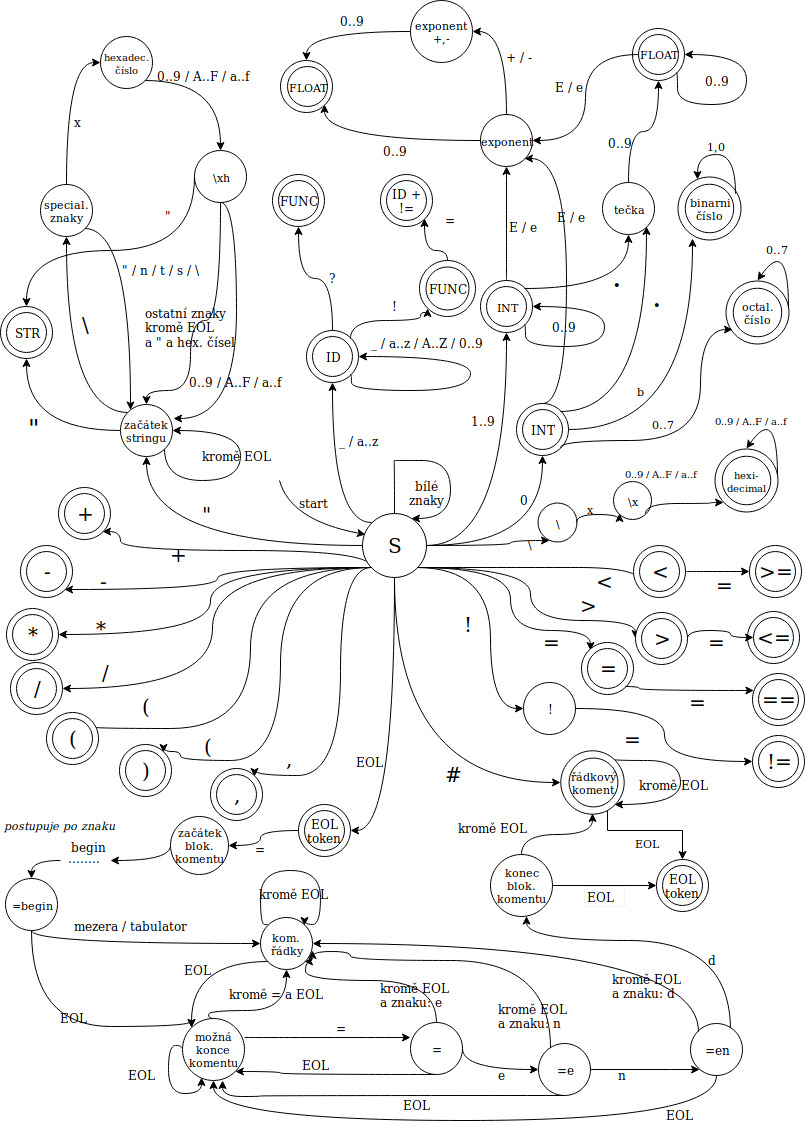
\includegraphics[scale=0.58]{KA.jpg}
\caption{Konečný automat}
\label{pic:1}
\end{center}
\end{figure}


\end{document}